\documentclass[aspectratio=169]{beamer}
\usetheme{metropolis}
\usepackage[utf8]{inputenc}
\usepackage{tikz}
\usetikzlibrary{positioning,fit,backgrounds,arrows.meta,decorations.pathreplacing}
\usepackage{booktabs}
\usepackage{array}

\definecolor{talkteal}{HTML}{1F6F78}
\definecolor{talkcoral}{HTML}{C05746}
\definecolor{talkgold}{HTML}{D1A344}
\setbeamercolor{palette primary}{bg=talkteal,fg=white}
\setbeamercolor{frametitle}{bg=talkteal,fg=white}
\setbeamercolor{progress bar}{fg=talkcoral,bg=talkteal!20}
\setbeamercolor{alerted text}{fg=talkcoral}

\title{Tensor Monte Carlo, Massively-Parallel RWS, and the Source Term Trick}
\subtitle{How \texttt{alan} does inference --- plus a look at some newer empirical follow-ups}
\author{}
\date{}

\begin{document}

\maketitle

\begin{frame}{Outline}
  \tableofcontents
\end{frame}

% =============================================================
\section{The problem}
% =============================================================

\begin{frame}{Why one sample per latent isn't enough}
  \begin{itemize}
    \item Standard importance sampling / VI: draw \emph{one} sample of the
      whole latent vector $z$ from $Q$, reweight by $p(z,x)/q(z)$.
    \item Better: draw $K$ \emph{whole-vector} samples (IWAE-style) and
      average --- tighter bound, lower variance, but cost is $O(K)$ per
      \emph{full model}, and you need $K$ large before it helps on models
      with many latents.
    \item \alert{What if we could afford $K$ samples \emph{per latent
      variable}, not per whole vector?} Naively that's $K^{\#\text{latents}}$
      combinations to consider --- looks hopeless.
  \end{itemize}
  \vfill
  This is the problem Tensor Monte Carlo, then Massively-Parallel RWS, and
  then the source term trick, solve in turn.
\end{frame}

\begin{frame}{Wake-Sleep, briefly}
  Classic wake-sleep (Hinton et al.) trains a generative model $P$ and a
  recognition/proposal model $Q$ together:
  \begin{center}
  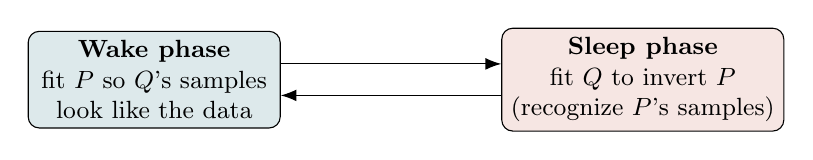
\begin{tikzpicture}[node distance=14mm,
      box/.style={draw,rounded corners,minimum width=32mm,minimum height=9mm,align=center,font=\small}]
    \node[box,fill=talkteal!15] (wake) {\textbf{Wake phase}\\ fit $P$ so $Q$'s samples\\ look like the data};
    \node[box,fill=talkcoral!15,right=28mm of wake] (sleep) {\textbf{Sleep phase}\\ fit $Q$ to invert $P$\\ (recognize $P$'s samples)};
    \draw[-{Latex[length=2mm]}] ([yshift=2mm]wake.east) -- ([yshift=2mm]sleep.west);
    \draw[-{Latex[length=2mm]}] ([yshift=-2mm]sleep.west) -- ([yshift=-2mm]wake.east);
  \end{tikzpicture}
  \end{center}
  \small\textbf{Reweighted Wake-Sleep (RWS)} improves the $Q$ update: instead
  of training $Q$ on $P$'s own samples, use self-normalized importance
  weights from $K$ samples of $Q$ to push $Q$ toward the \emph{true
  posterior} directly.
\end{frame}

% =============================================================
\section{Tensor Monte Carlo}
% =============================================================

\begin{frame}{Tensor Monte Carlo (Aitchison, 2019)}
  The key move that makes ``$K$ samples per latent'' tractable:
  \begin{itemize}
    \item Draw $K$ candidate values for \emph{each} latent variable
      separately, not $K$ whole-vector samples.
    \item Most latents only interact with a handful of neighbours in the
      model's dependency graph (plates, conditional independence).
    \item So the $K^{\#\text{latents}}$ sum factorizes into a sequence of
      small tensor contractions (like \texttt{einsum}) that follow the
      graph structure --- cost becomes polynomial in $K$, not exponential.
  \end{itemize}
\end{frame}

\begin{frame}{Why this matters}
  \begin{center}
  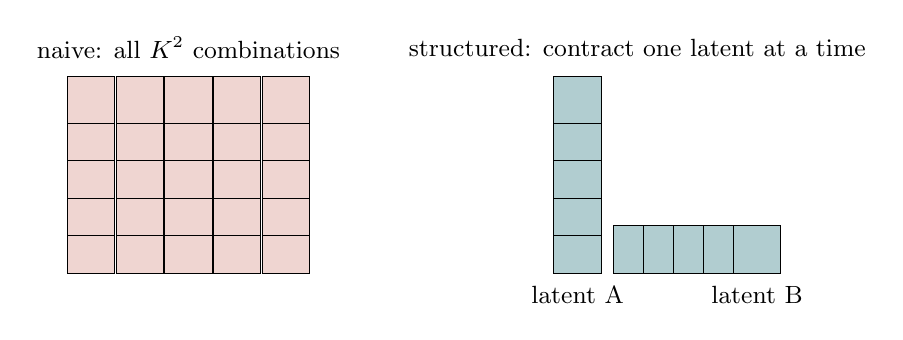
\begin{tikzpicture}[scale=0.95,
      cell/.style={draw,minimum size=6mm}]
    % naive grid
    \node at (0,3.0) {\small naive: all $K^2$ combinations};
    \foreach \i in {0,...,4}{
      \foreach \j in {0,...,4}{
        \node[cell,fill=talkcoral!25] at (\i*0.65-1.3,\j*0.5+0.3) {};
      }
    }
    % structured contraction
    \node at (6,3.0) {\small structured: contract one latent at a time};
    \foreach \j in {0,...,4}{
      \node[cell,fill=talkteal!35] at (5.2,\j*0.5+0.3) {};
    }
    \foreach \i in {0,...,4}{
      \node[cell,fill=talkteal!35] at (\i*0.4+6.0,0.3) {};
    }
    \node[font=\small] at (5.2,-0.3) {latent A};
    \node[font=\small] at (7.6,-0.3) {latent B};
  \end{tikzpicture}
  \end{center}
  \vfill
  Same $K$, same model --- but reducing latent by latent (following the
  graph) instead of enumerating the full product turns an exponential sum
  into a polynomial one.
\end{frame}

\begin{frame}{What TMC gives you --- and doesn't}
  \begin{itemize}
    \item[\alert{+}] A much lower-variance, $K$-per-latent marginal
      likelihood estimator, at polynomial cost.
    \item[\alert{--}] On its own, it's just an estimator --- no prescription
      for \emph{training} $P$ and $Q$ together, and no cheap way to get
      posterior samples/moments back out afterward.
  \end{itemize}
  \vfill
  \textbf{Massively-Parallel Reweighted Wake-Sleep} (Heap et al., UAI 2023)
  turns this estimator into a full training algorithm.
\end{frame}

% =============================================================
\section{Massively-Parallel RWS}
% =============================================================

\begin{frame}{The estimator: $P_{\text{MP}}(z)$}
  For each latent, draw $K$ particles from $Q$; contract following the plate
  structure (as above) to get a single scalar:
  \[
    \hat{P}_{\text{MP}}(x) \;=\; \text{(TMC-style contraction of } p(z,x)/q(z)
    \text{ over all latents' } K \text{ particles)}
  \]
  \begin{itemize}
    \item \alert{Unbiased}: $\mathbb{E}[\hat P_{\text{MP}}(x)] = p(x)$, the
      true marginal likelihood --- proved directly, not just assumed.
    \item This single fact is what later makes \emph{exact} MCMC schemes
      (Particle MCMC) possible on top of this machinery --- more on that at
      the end.
  \end{itemize}
\end{frame}

\begin{frame}{Two updates, one estimator}
  \begin{columns}[T]
    \begin{column}{0.48\textwidth}
      \begin{block}{Wake phase (update $P$)}
        Maximize $\log \hat P_{\text{MP}}(x)$ --- the massively-parallel
        analogue of the IWAE bound (more on this next).
      \end{block}
    \end{column}
    \begin{column}{0.48\textwidth}
      \begin{block}{Sleep phase (update $Q$)}
        Self-normalize the same per-latent importance weights, use them to
        push $Q$ toward the true posterior --- the ``reweighted'' part of
        RWS, now done per-latent instead of per-whole-vector.
      \end{block}
    \end{column}
  \end{columns}
  \vfill
  Both updates reuse \emph{the same} $K$-particle contraction --- no
  separate machinery for training $P$ vs. $Q$.
\end{frame}

% =============================================================
\section{The MP-IW bound}
% =============================================================

\begin{frame}{From IWAE to Massively-Parallel Importance-Weighted}
  \begin{itemize}
    \item The IWAE bound: average $K$ \emph{whole-vector} importance
      weights, take the log --- gets tighter (closer to $\log p(x)$) as $K$
      grows.
    \item \textbf{MP-IW}: the same idea, but the $K$ particles are per
      latent, contracted via the plate structure --- so the bound gets
      tighter per unit of \emph{actual} compute, not just per unit of $K$.
    \item Practically: many more effective ``combinations'' are being
      averaged over for the same memory/compute budget.
  \end{itemize}
  \vfill
  \small This bound is exactly what \texttt{alan} exposes as
  \texttt{sample.elbo\_rws()} / \texttt{elbo\_vi()} in the code.
\end{frame}

% =============================================================
\section{The source term trick}
% =============================================================

\begin{frame}{The remaining problem}
  MP-RWS gives you a great scalar (the bound) and gradients for training.
  \vfill
  But once you have a trained $P,Q$: how do you get
  \begin{itemize}
    \item posterior \textbf{samples},
    \item posterior \textbf{marginals} (the per-latent weight distribution
      over its $K$ particles),
    \item posterior \textbf{moments} (means, variances, covariances)
  \end{itemize}
  back out, \alert{without writing a bespoke resampling algorithm for every
  different plate topology}?
\end{frame}

\begin{frame}{The trick}
  \emph{Using Autodiff to Estimate Posterior Moments, Marginals and Samples}
  (Bowyer, Heap \& Aitchison, UAI 2024):
  \begin{enumerate}
    \item Add an auxiliary \textbf{source term} $J$ into the log joint,
      additively, before running the \emph{exact same} $K$-dim contraction
      used to compute the bound.
    \item That contraction now computes a scalar $L(J)$ instead of just
      $L(0)$.
    \item \alert{Differentiate $L(J)$ w.r.t.\ $J$, at $J=0$, using ordinary
      autodiff.} The derivative \emph{is} the marginal / moment you wanted.
  \end{enumerate}
  \vfill
  \small Exactly the same move as getting moments from
  $\partial \log Z[J] / \partial J$ for a log-partition function with an
  external source $J$ --- a very old idea in statistical physics and
  exponential families, applied here to a Monte Carlo estimator instead of
  an analytic one.
\end{frame}

\begin{frame}{Why this is the elegant part}
  \begin{itemize}
    \item No new algorithm per quantity --- \texttt{alan} computes
      posterior samples, marginals, \emph{and} moments through literally the
      same code path that computes the bound.
    \item Works uniformly across arbitrarily nested plates --- the
      contraction already handles that; the source term rides along for
      free.
    \item It's autodiff doing the bookkeeping that would otherwise be a
      hand-written, model-specific resampling routine.
  \end{itemize}
\end{frame}

\begin{frame}[fragile]{This is really in the code}
  From \texttt{alan}'s \texttt{Sample.py} (lightly trimmed):
  \begin{center}
  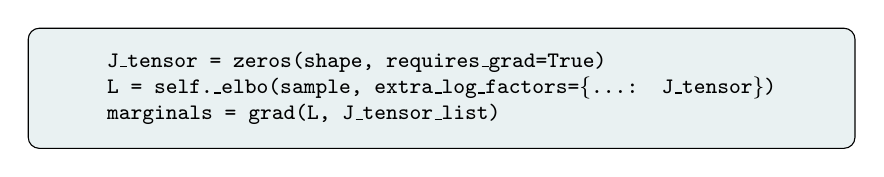
\begin{tikzpicture}[node distance=3mm,
      box/.style={draw,rounded corners,align=left,font=\footnotesize\ttfamily,minimum width=105mm,inner sep=3mm}]
    \node[box,fill=talkteal!10] (a) {J\_tensor = zeros(shape, requires\_grad=True)\\
      L = self.\_elbo(sample, extra\_log\_factors=\{...: J\_tensor\})\\
      marginals = grad(L, J\_tensor\_list)};
  \end{tikzpicture}
  \end{center}
  \vfill
  \begin{itemize}
    \item \texttt{J\_tensor} starts at all zeros --- it doesn't change what
      \texttt{L} evaluates to.
    \item But differentiating \texttt{L} through it gives back exact
      per-particle marginal weights, for whichever latent(s) \texttt{J} was
      attached to.
  \end{itemize}
\end{frame}

% =============================================================
\section{How it fits together}
% =============================================================

\begin{frame}{The whole picture}
  \begin{center}
  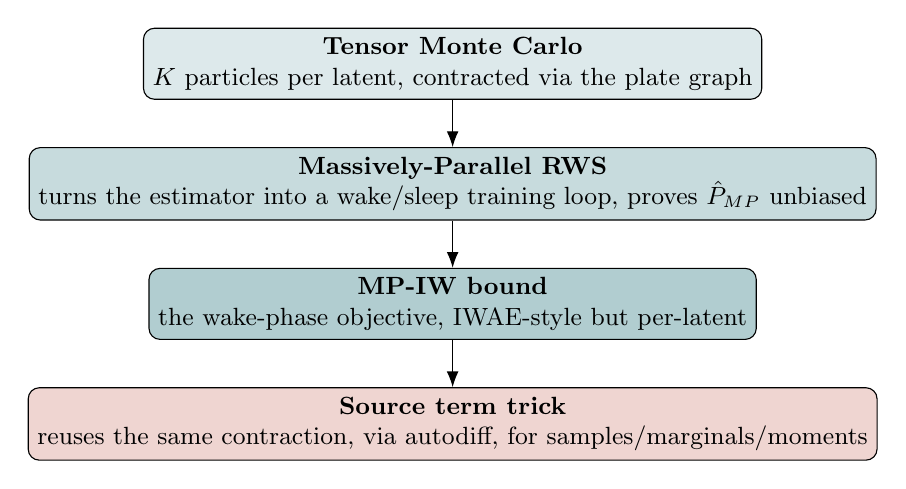
\begin{tikzpicture}[node distance=6mm,
      box/.style={draw,rounded corners,minimum width=70mm,minimum height=8mm,align=center,font=\small}]
    \node[box,fill=talkteal!15] (tmc) {\textbf{Tensor Monte Carlo}\\ $K$ particles per latent, contracted via the plate graph};
    \node[box,fill=talkteal!25,below=of tmc] (mprws) {\textbf{Massively-Parallel RWS}\\ turns the estimator into a wake/sleep training loop, proves $\hat P_{\text{MP}}$ unbiased};
    \node[box,fill=talkteal!35,below=of mprws] (mpiw) {\textbf{MP-IW bound}\\ the wake-phase objective, IWAE-style but per-latent};
    \node[box,fill=talkcoral!25,below=of mpiw] (source) {\textbf{Source term trick}\\ reuses the same contraction, via autodiff, for samples/marginals/moments};
    \draw[-{Latex[length=2mm]}] (tmc) -- (mprws);
    \draw[-{Latex[length=2mm]}] (mprws) -- (mpiw);
    \draw[-{Latex[length=2mm]}] (mpiw) -- (source);
  \end{tikzpicture}
  \end{center}
\end{frame}

% =============================================================
\section{Newer empirical follow-ups}
% =============================================================

\begin{frame}{What I've been doing on top of this}
  \small
  All still grounded in the same $\hat P_{\text{MP}}(z)$ estimator and the
  source term trick above. Four quick results:
  \begin{enumerate}
    \item Does MP-IS actually beat plain self-normalized IS / catch up to
      HMC in practice?
    \item A bug hunt that uncovered a real fact about how \texttt{alan}'s
      plate reduction works.
    \item Where jackknife bias-correction does and doesn't help.
    \item Two early prototypes: a general debiasing scheme (BR-SNIS), and
      exact inference via Particle Gibbs --- both enabled directly by
      $\hat P_{\text{MP}}(z)$'s unbiasedness.
  \end{enumerate}
\end{frame}

\begin{frame}{1: MP-IS vs.\ Global-IS vs.\ HMC}
  \begin{center}
    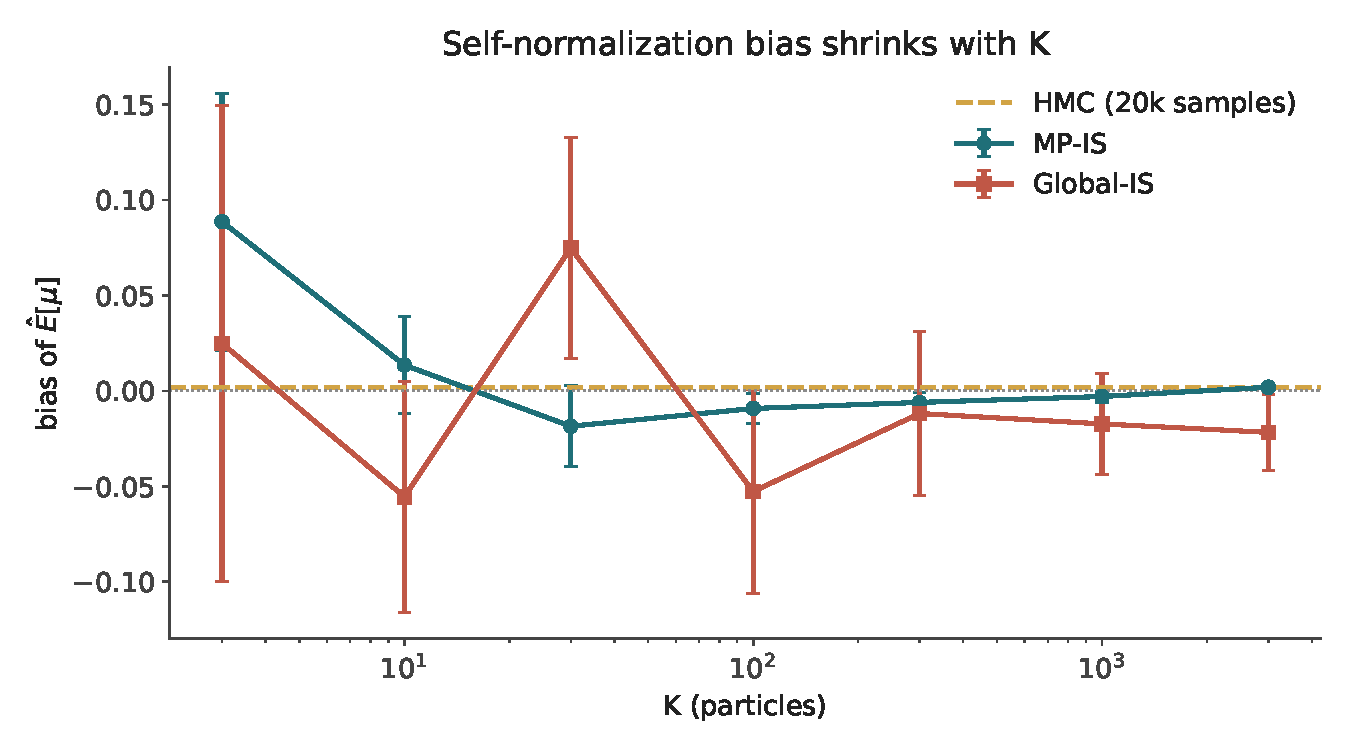
\includegraphics[width=0.66\textwidth]{figures/bias_vs_K.pdf}
  \end{center}
  \small MP-IS's bias shrinks toward HMC's own (tiny) bias as $K$ grows;
  Global-IS (whole-vector, no plate exploitation) is 5--10$\times$ worse at
  matched $K$ throughout.
\end{frame}

\begin{frame}{2 \& 3: a bug hunt, and where jackknife helps}
  \begin{itemize}
    \item A hand-rolled reimplementation didn't match \texttt{alan}'s own
      output --- traced to a genuine, previously undocumented fact: each
      plate element reduces its own $K$ particles \emph{independently}
      before summing across the plate (an extra Rao--Blackwellization the
      plate structure buys for free).
    \item Marginal ESS (via the source term trick's marginals) is bounded by
      $K$ and uneven across plate replicates --- up to $4\times$ spread at
      matched $K$.
    \item Delete-one jackknife removes most of the small-$K$ bias for
      variables that reduce via a flat ratio, but \alert{not} for variables
      reduced through a nested per-plate-element step --- a precise,
      structural distinction, not a coincidence.
  \end{itemize}
\end{frame}

\begin{frame}{4: two prototypes enabled by $\hat P_{\text{MP}}$'s unbiasedness}
  \begin{columns}[T]
    \begin{column}{0.48\textwidth}
      \textbf{BR-SNIS} (chain-recycling debiasing): only competitive with
      MP-IS's own efficiency once pointed \emph{at} the already
      plate-reduced ratio --- a flat version loses badly.
    \end{column}
    \begin{column}{0.48\textwidth}
      \textbf{Particle Gibbs / PGAS}: pins a reference trajectory using
      $\hat P_{\text{MP}}$'s unbiasedness for exact posteriors. Ancestor
      sampling (PGAS) gives a measured 74$\times$ mixing improvement over
      plain Particle Gibbs at matched $K$.
    \end{column}
  \end{columns}
  \vfill
  \small Both are toy-model prototypes, not yet integrated into
  \texttt{alan}'s core --- write-ups and numbers are in the design doc for
  whoever picks this up next.
\end{frame}

% =============================================================
\section*{Wrap-up}
% =============================================================

\begin{frame}{Summary}
  \begin{itemize}
    \item TMC makes $K$-per-latent tractable by contracting along the plate
      graph.
    \item MP-RWS turns that estimator into a training algorithm, and proves
      it unbiased.
    \item The MP-IW bound is the resulting wake-phase objective --- IWAE,
      scaled per latent instead of per whole vector.
    \item The source term trick gets samples/marginals/moments out of the
      \emph{same} computation, via autodiff, for free.
    \item That unbiasedness is now being put to work: empirical bias
      checks, a real reduction-order finding, and two exact/debiasing
      prototypes building directly on it.
  \end{itemize}
\end{frame}

\begin{frame}[standout]
  Questions
\end{frame}

\end{document}
